\section{Learning to Learn from Weak Supervision, by Full Supervision}
\label{sec:meta_learning}
Using weak or noisy supervision is a straightforward approach to increase the size of the training data. This is usually done by pre-training the network on a large set of weakly labeled data and fine tuning it with strong labels~\citep{Dehghani:2017:SIGIR,Severyn:2015:SIGIR}. 
However, these two independent stages do not leverage the full capacity of information from the small set of strong labels, as it can be useful for learning how to learn from the weak labels.  In particular, in the pre-training stage, we have to learn from labels of variable quality without any control over how these labels contribute to the learning process.

In this section, we address the first research question of this chapter:
\resq{c5.1}

We introduce a semi-supervised method that leverages a small amount of data with strong labels to improve the learning from a large amount of data with weak labels. This model, in fact, offers learning from \emph{Controlled Weak Supervision} and we refer to it by \emph{\cws} in the rest of this chapter.
%
\cws has three main components:
(1) A \wa, which can be a heuristic model, a weak or biased classifier, or even a human via crowd-sourcing and it is employed to annotate a massive amount of unlabeled data, 
(2) a \tnet, which uses a large set of weakly annotated samples by the \wa to learn the main task, 
(3) and a \cnet, which is trained on a small set with strong labels to estimate confidence scores for samples annotated by the \wa. 

The confidence scores estimated by the \cnet define the magnitude of the weight updates applied to the \tnet during training. This way, the \cnet helps the \tnet to avoid the mistakes of its teacher, i.e., \wa, by down-weighting the weight updates from weak labels that do not look reliable according to \cnet.
%
\cws, in fact, employs the teacher-student paradigm in which the \tnet (student) and the \cnet (teacher) are trained jointly in a multi-task fashion and they share parameters of the representation learning layer to share their understanding of the data.

From a meta-learning perspective~\citep{Andrychowicz:2016,Finn2017:ICML,Ravi:2016}, the goal of the \cnet\ ---as the meta-learner--- trained jointly with the \tnet\ ---as the learner--- is to calibrate the learning rate of the \tnet for each sample in the batch. I.e., the weights $\pmb{w}$ of the \tnet $f_w$ at step $t+1$ are updated as follows:
\begin{equation}
\pmb{w}_{t+1} = \pmb{w}_t - \frac{\eta_t}{b}\sum_{i=1}^b c_{\theta}(x_i, \tilde{y}_i)  \nabla \mathcal{L}(f_{\pmb{w_t}}(x_i), \tilde{y}_i),
%+ \nabla \mathcal{R}(\pmb{w_t})
\end{equation}
where $\eta_t$ is the global learning rate, $\mathcal{L}(\cdot)$ is the loss of predicting $\hat{y}=f_w(x_i)$ for an input $x_i$ when $\tilde{y}$ is the weak label; $c_\theta(\cdot)$ is a scoring function learned by the \cnet taking input instance $x_i$ and its noisy label $\tilde{y}_i$. Thus, we can effectively control the contribution to the parameter updates for the \tnet from weakly labeled samples based on how reliable their labels are according to the \cnet (learned on a small supervised data).

Our setup requires running a \wa to label a large amount of unlabeled data, which is done at pre-processing time. For many tasks, it is possible to use a simple heuristic, a rule-based function, or implicit human feedback to generate weak labels. This set is then used to train the \tnet.  
In contrast, a small expert-labeled set is used to train the \cnet, which estimates how good the weak annotations are, i.e., controls the effect of weak labels on updating the parameters of the \tnet.

\cws allows learning different types of neural architectures and various tasks, where a meaningful \wa is available. 
Later in this chapter we study the performance of \cws by focusing on two applications: sentiment classification and document ranking. 

\subsection{Learning from Controlled Weak Supervision}
\label{sec:method}
% \label{sec:generalarchitecture}
\begin{figure}[!htbp]%
    % \makebox[\textwidth][c]{
    \centering
    \begin{subfigure}[t]{\textwidth}
        \centering
        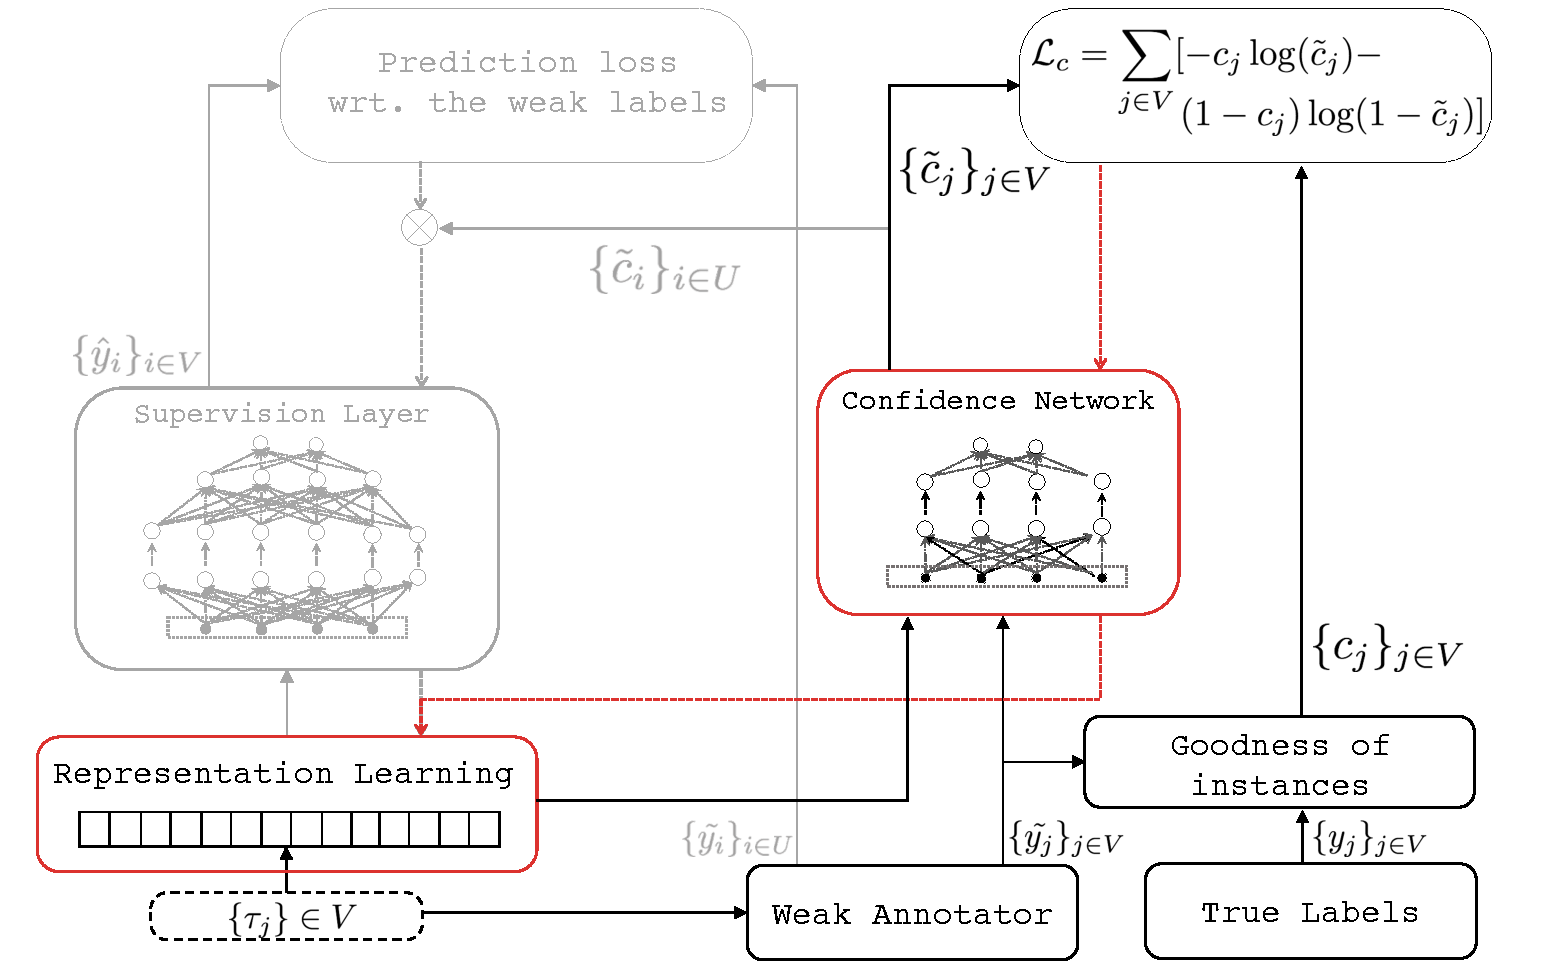
\includegraphics[width=\textwidth]{03-part-02/chapter-05/figs_and_tables/fig_cws_train_v.pdf}
        \caption{\label{fig:train_u}\footnotesize{Full Supervision Mode: Training on batches with strong labels.}}
    \end{subfigure}%
    \vfill
    \vspace{20pt}
    \begin{subfigure}[t]{\textwidth}
        \centering
        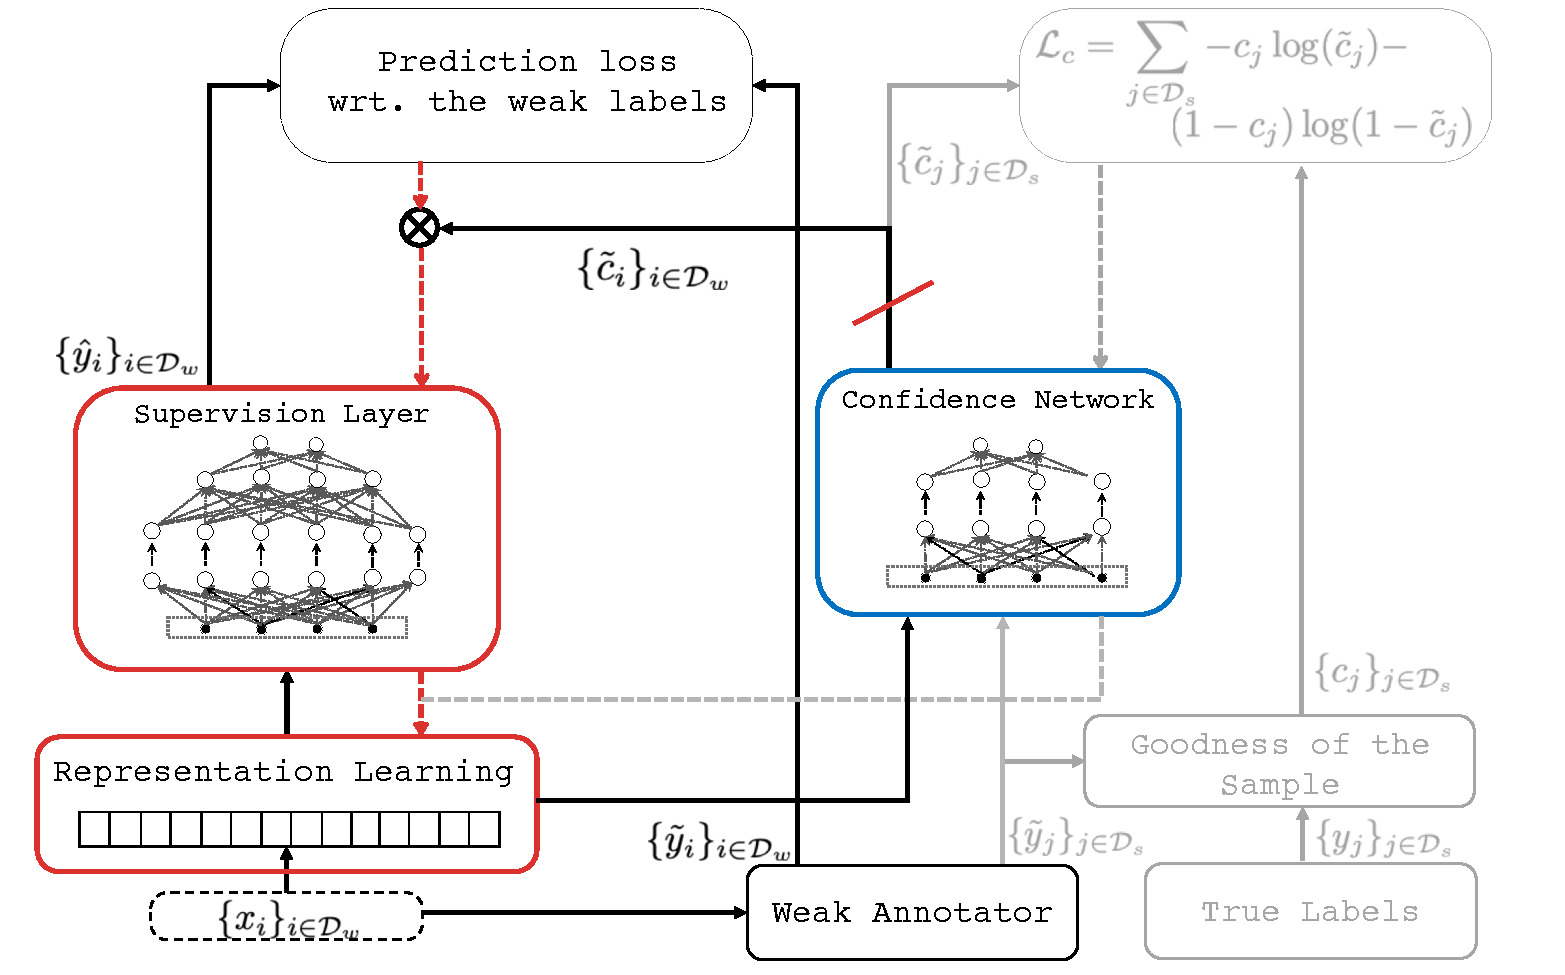
\includegraphics[width=\textwidth]{03-part-02/chapter-05/figs_and_tables/fig_cws_train_u.pdf}
        \caption{\label{fig:train_v}\footnotesize{Weak Supervision Mode: Training on batches with weak labels.}}
    \end{subfigure}%
    % }
    \caption{Learning from controlled weak supervision: Our proposed multi-task network for learning a target task in a semi-supervised fashion, using a large amount of weakly labeled data and a small amount of data with strong labels.
    %
    Faded parts of the network are disabled during the training in the corresponding mode. Red-dotted arrows show gradient propagation. Parameters of the parts of the network in red frames get updated in the backward pass, while parameters of the network in blue frames are fixed during training. (Best viewed in color.)}
    \label{fig:model_cws}
\end{figure}

In the following, we describe our recipe for training a multi-task neural network that jointly learns the confidence score of weakly labeled samples and the main task using controlled supervised signals. The high-level representation of the model is shown in Figure~\ref{fig:model_cws}. 

Our model comprises a \wa and two neural networks: the \cnet and the \tnet. Formally speaking, the goal of the \wa is to \emph{provide weak labels} $\tilde{y}_i$ for all the instances $x_i \in \mathcal{D}_w \cup \mathcal{D}_s$. We have the assumption that $\tilde{y}_i$ provided by the \wa are imperfect estimates of strong labels $y_i$, where $y_i$ are available for the set $\mathcal{D}_s$, but not for the set $\mathcal{D}_w$.

The goal of the \cnet is to \emph{estimate the confidence score} $\tilde{c}_j$ of training samples. It is learned on samples from the training set $\mathcal{D}_s$, i.e a set of input $x_j$ and its strong label $y_j$ as well its weak label,  $\tilde{y}_j$,  that is annotated by the \wa.
The score $\tilde{c}_j$ is then used to control the effect of weakly labeled samples on updating the parameters of the \tnet in the backward pass of backpropagation.

The \tnet is in charge of \emph{handling the main task} we want to learn, or in other words, approximating the underlying function that predicts the correct labels. 
Given a data instance, $x_i$ and its weak label $\tilde{y}_i$ from the training set $\mathcal{D}_w$, the \tnet aims to predict the label $\hat{y}_i$. 
The \tnet parameter updates are based on noisy labels assigned by the \wa, but the magnitude of the gradient update is based on the output of the \cnet. 

Both networks are trained in a multi-task fashion alternating between the \emph{full supervision} and the \emph{weak supervision} mode.  
In the \emph{full supervision} mode, the parameters of the \cnet get updated using instances from training set $\mathcal{D}_s$.  
As depicted in Figure~\ref{fig:train_v}, each training instance is passed through the representation layer mapping inputs to vectors. These vectors are concatenated with their corresponding weak labels $\tilde{y}_j$ generated by the \wa.
The \cnet, which is a fully connected feedforward network with sigmoid as the output layer, estimates $\tilde{c}_j$ that is the probability of taking data instance $j$ into account for training the \tnet.

In the \emph{weak supervision} mode, the parameters of the \tnet are updated using the training set $\mathcal{D}_w$.
As shown in Figure~\ref{fig:train_u}, each training instance is passed through the same representation learning layer and is then processed by the supervision layer which is a part of the \tnet predicting the label for the main task. 
%
We also pass the learned representation of each training instance along with its corresponding label generated by the \wa to the \cnet to estimate the \emph{confidence score} of the training sample, i.e., $\tilde{c}_i$. 
The confidence score is computed for each sample from the training set $\mathcal{D}_w$. These confidence scores are used to weight the gradient updating \tnet parameters or in other words the step size during back-propagation. 

It is noteworthy that the representation layer is shared between both networks.  Thus, besides the regularization effect of updating the parameters of this layer with respect to two loses, sharing this layer helps the \cnet to use the representation learned based on a samples of the set $\mathcal{D}_w$ as a rather large set, as well as the \tnet to utilize the information from samples of the set $\mathcal{D}_s$, as a rather clean set. Most importantly, sharing this layer lets the \cnet and the \tnet to have the same point of view on data points.

\subsection{Training the Learner and the Meta-Learner}
\label{sec:modeltraining}
Here, we explain how we train \cws in which we jointly update the parameters of the \tnet, the learner and the \cnet, the meta-learner. 
Our optimization objective is composed of two terms: (1) the \cnet loss $\mathcal{L}_c$, which captures the quality of the output from the \cnet and (2) the \tnet loss $\mathcal{L}_t$, which expresses the quality for the main task. 

Both networks are trained by alternating between the \emph{weak supervision} and the \emph{full supervision} mode:


\textbf{Full Supervision Mode}: in this mode, the parameters of the \cnet are updated using training instances drawn from training set $\mathcal{D}_s$. We use the cross-entropy loss function for the \cnet to capture the difference between the predicted confidence score of sample $j$, i.e., $\tilde{c}_j$ and the target score $c_j$:
\begin{equation}
% \nonumber
\mathcal{L}_c = \sum_{j\in \mathcal{D}_s} -  c_j \log(\tilde{c}_j) - (1-c_j) \log(1-\tilde{c}_j).
\end{equation}
%given that $c_j$ is not a probability I'm wondering if we can call this loss a cross-entropy --- it only makes sense if $c_j$ is a probability of binary event. Possibly, it's common to use in IR, but i've never seen it used like this on real-valued scores.} 
The target score $c_j$ indicates how similar the strong and the weak labels are, and it is calculated with respect to the main task. 

\textbf{Weak Supervision Mode}: In this mode, the parameters of the \tnet are updated using training instances from $\mathcal{D}_w$. We use a weighted loss function, $\mathcal{L}_t$, to capture the difference between the predicted label $\hat{y}_i$ by the \tnet and target label $\tilde{y}_i$:
\begin{equation}
% \nonumber
\mathcal{L}_t = \sum_{i\in U} \tilde{c}_i \mathcal{L}_i,
\end{equation}
where $\mathcal{L}_i$ is the task-specific loss on training sample $i$ and $\tilde{c}_i$ is the confidence score of the weakly annotated sample $i$, estimated by the \cnet.
Note that $\tilde{c}_i$ is treated as a constant during the weak supervision mode and there is no gradient propagation to the \cnet in the backward pass (as depicted in Figure~\ref{fig:train_u}). 

\medskip
We minimize two loss functions jointly by randomly alternating between full and weak supervision modes (for example, using a 1:10 ratio).
During training and based on the chosen supervision mode, we sample a batch of training instances from $\mathcal{D}_s$ with replacement or from $\mathcal{D}_w$ without replacement (since $\mathcal{D}_w$ can be very large). Since in our setups usually $|\mathcal{D}_w| \gg |\mathcal{D}_s|$, the training process oversamples the instance from $\mathcal{D}_s$. 

The key point here is that the ``main task'' and ``confidence scoring'' task are always defined to be close tasks and sharing representation will benefit the confidence network as a kind of implicit data augmentation to compensate the small amount of data with strong labels.
Besides, updating the representation layer with respect to the loss of the other network acts as a regularization for each of these networks and helps generalization for both target and confidence network and consequently less chance for overfitting.

% We also investigated other possible setups or training scenarios. For instance, we tried updating the parameters of the supervision layer of the \tnet using also data with strong labels. Or instead of using alternating sampling, we tried training the \tnet using controlled weak supervision signals after the \cnet is fully trained.
% As shown in the experiments the architecture and training strategy described above provide the best performance.

\medskip
In this section, we introduced an approach that can meta-learn the quality of labels as confidence scores, jointly with the main task at hand, when learning with weakly labeled samples that have variable qualities. 
We showed that we can incorporate the estimated confidence scores associated with each weakly labeled sample to control the magnitude of the parameter updates during training based on the quality of that sample. 
In the next section, we introduce another approach that can estimate the quality of samples and regulate the learning process based on it.